\title{ 15. Kuželosečky - kružnice, elipsa}
\author{Aneta Foralová}
\date{30.4.2025}

\maketitle

\section{Kružnice, elipsa}


\begin{figure}[H]
        \centering
        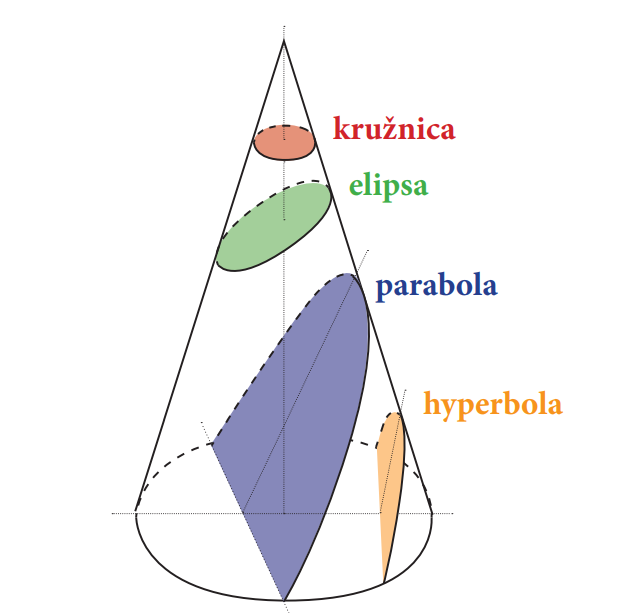
\includegraphics[width=0.3\linewidth]{img/14_kuzelosecky.png}
        \caption{Kuželosečky} 
        \label{fig:enter-label}
    \end{figure}    

\subsection{Definice}
    Pojem \textbf{KUŽELOSEČKY} vznikl jako název množin bodů v prostoru, které lze získat jako průniky roviny a kuželové plochy.\\
    
    Nechť je dán v rovině $E_2$ bod $S$ a číslo $r \in \mathbb{R}$, $r > 0$. \textbf{KRUŽNICE} je množina všech bodů v rovině, které leží ve stejné vzdálenosti, označované jako poloměr, od pevně daného bodu, zvaného střed.\\
    
    Nechť jsou dány v rovině $E_2$ dva různé body $F$ a $G$. \textbf{ELIPSA} je množina všech bodů v rovině, které mají stálý součet vzdáleností ($2a$) od dvou pevně daných bodů, tzv. ohnisek.\\

    Je-li střed elipsy bod $S[0;0]$ poté platí:\\
    Číslo  $e > 0$ se nazývá \textbf{excentricita elipsy} a platí: $e^2 = a^2 - b^2 , a > b$\\
    Body $A[a;0], B[-a;0]$ se nazývají \textbf{hlavní vrcholy elipsy}\\ $a>0$ se nazývá \textbf{hlavní poloosa elipsy}\\ Body $C[0;b], D[0;-b]$ se nazývají \textbf{vedlejší vrcholy elipsy}\\$b>0$ se nazývá \textbf{vedlejší poloosa elipsy}\\
    

    \begin{figure}[H]
        \centering
        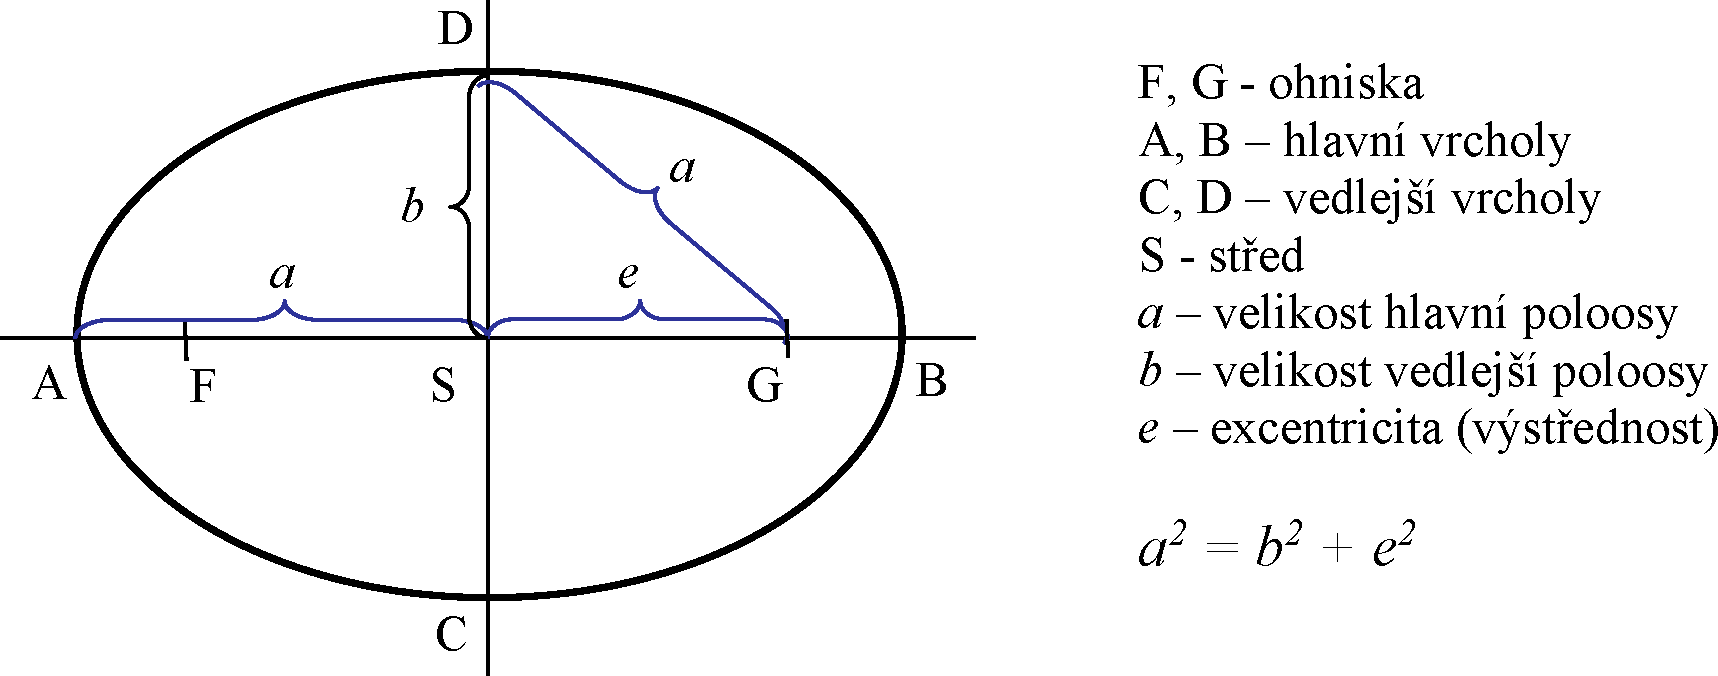
\includegraphics[width=0.6\linewidth]{img/14_elipsa1.png}
        \caption{Elipsa} 
        \label{fig:enter-label}
    \end{figure}    

\subsection {Středové a obecné rovnice}
    Obecnou rovnici kuželosečky získáme ze středové rovnice provedením operací ve středové rovnici a zavedením nových konstant\\
    Středovou rovnici kuželosečky získáme z obecné rovnice doplněním na čtverec
\subsubsection{Kružnice}
    Je-li S[0;0] středová rovnice kružnice je: 
    $$
    x^2 + y^2 = r^2
    $$
    A je-li S[$m;n$] a $r>0$, je středová rovnice kružnice 
    $$
    (x-m)^2 + (y-n)^2 = r^2
    $$
    Obecná rce kružnice je 
    $$
    x^2 + y^2 - 2mx - 2ny+q=0,
    $$
    kde $p=m^2 + n^2-r^2$\\
    \vspace{1em} 
    
    \begin{figure}[H]
        \centering
        \includegraphics[width=0.3\linewidth]{img/14_kružnice.png}
        \caption{Kružnice} 
        \label{fig:enter-label}
    \end{figure}

\subsubsection{Elipsa}
    Jeli S[0;0] a elipsa je umístěna horizontálně tedy A[$a$;0] a B[$-a$;0] pak středová rovnice elipsy je  
    $$
    \frac{x^2}{a^2} + \frac{y^2}{b^2}=1
    $$\\ 
    \vspace{1em}
    
    \begin{figure}[H]
        \centering
        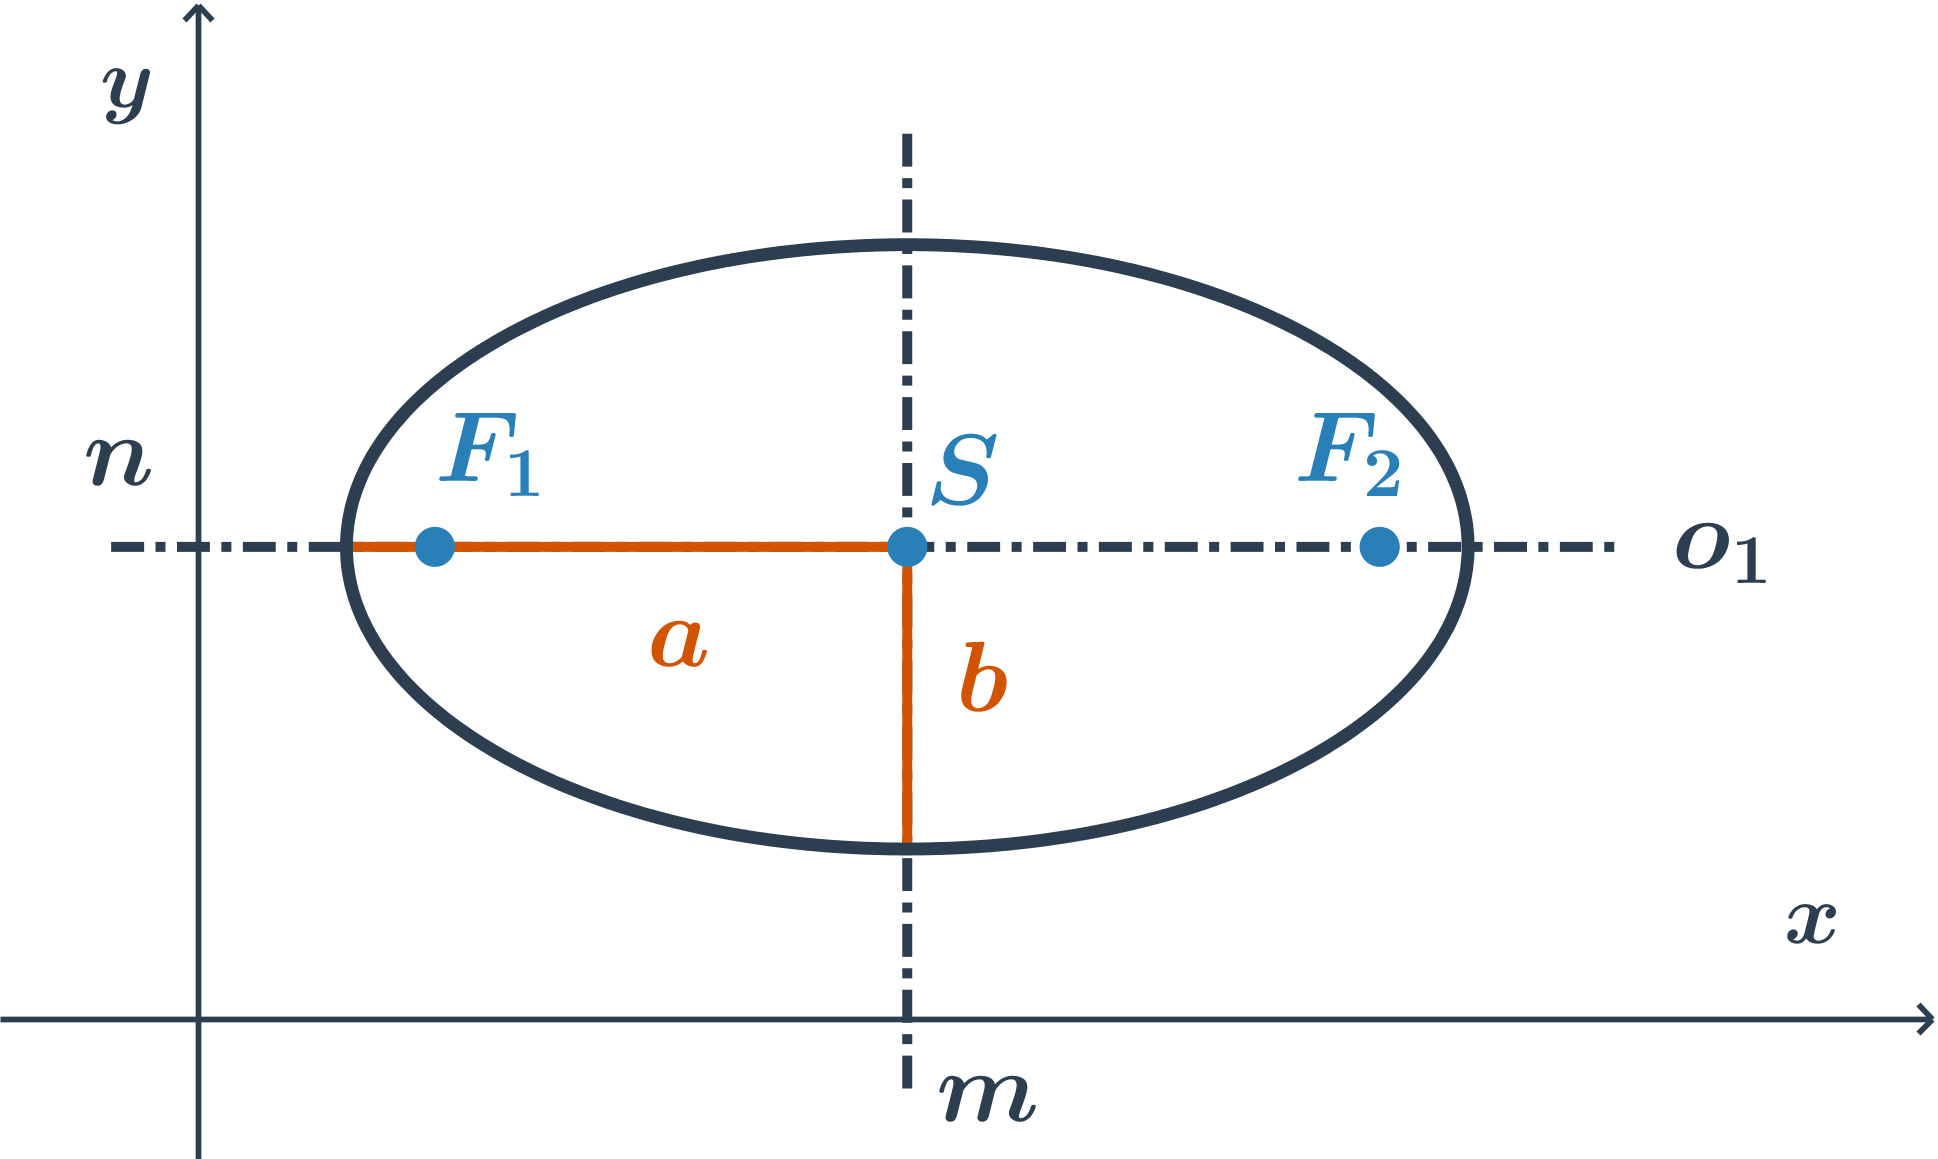
\includegraphics[width=0.5\linewidth]{img/14_elipsa3.png}
        \caption{Elipsa s hlavní poloosou x} 
        \label{fig:enter-label}
    \end{figure}
    
  
    \vspace{1em}
    Jeli S[0;0] a elipsa je umístěna vertikálně tedy A[0;$a$] a D[$b$;0], $a > b$ pak středová rovnice elipsy je  
    $$
    \frac{x^2}{b^2} + \frac{y^2}{a^2}=1
    $$\\
    \vspace{1em} 
    
    \begin{figure}[H]
        \centering
        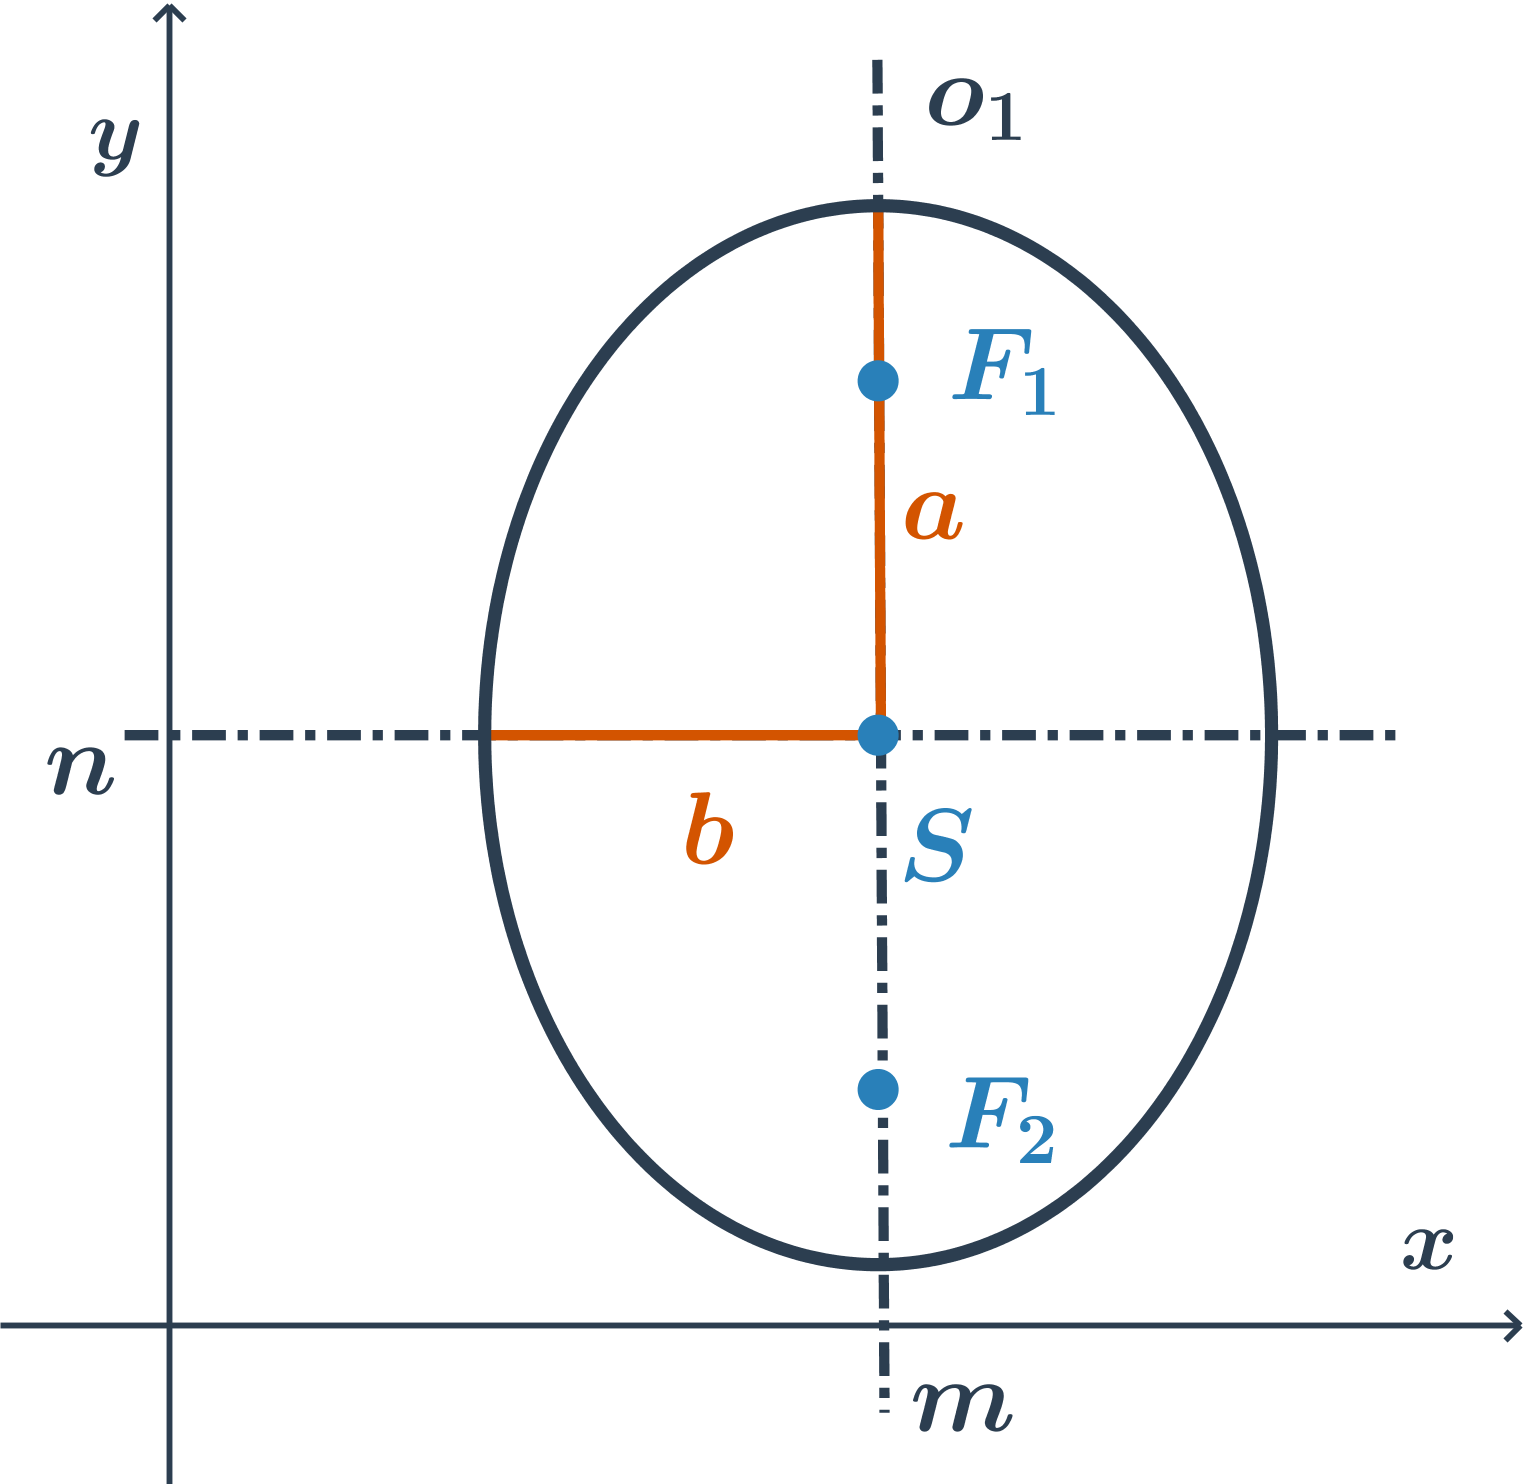
\includegraphics[width=0.3\linewidth]{img/14_elipsa 2.png}
        \caption{Elipsa s hlavní poloosou y} 
        \label{fig:enter-label}
    \end{figure}
    
    \vspace{1em}
    Je-li $S[m;n], a>0 $ , $ b>0 $ , $ a>b$ je středová rovnice elipsy: 
    $$
    \frac{(x-m)^2}{a^2} + \frac{(y-n)^2}{b^2}=1
    $$ 
    Obecná rce elipsy je: $px^2+qy^2+2rx+2sy+t=0$, kde $pq>0$
\subsection{Vzájemná poloha kuželosečky a bodu}
    Nechť je dána obecná rovnice kuželosečky a bod $A[x_A,y_A]$. Označíme si levou stranu obecné rovnice kuželosečky $f(x,y)$ pro každý bod kuželosečky a dosadíme souřadnice bodu $A[x_A,y_A]$ a pro jednotlivé kuželosečky platí: \begin{itemize}
        \item $A$ je bodem kuželosečky právě tehdy když $f(x_A,y_a)=0$
        \item $A$ je vnějším bodem kuželosečky právě když $f(x_A,y_a)>0$
        \item $A$ je vnitřním bodem kuželosečky právě když $f(x_A,y_a)<0$
    \end{itemize}
\subsection{Vzájemná poloha kuželosečky a přímky}
    Vzájemnou polohu kuželosečky a přímky určujeme tak, že hledáme jejich společné body. Analyticky to znamená, že hledáme řešení soustavy lineární rce (přímka) a kvadratické rce (kuželosečka) o dvou neznámých. To nakonec vede k řešení kvadratické rce o jendé neznáme. Ta může mít: \begin{itemize}
        \item Pro $D>0$ - dva společné body tj. sečna
        \item Pro $D=0$ - jedno řešení tj. tečna
        \item Pro $D<0$ - žádné řešení tj. vnější přímka
    \end{itemize}
\subsection{Vzájemná poloha kuželoseček}
    Vzájemná poloha kuželoseček se zkoumá opět tak, že se hledají společné body, analyticky to znamená, že se řeší soustava dvou kvadratických rovnic o dvou neznámých
